%%%%%%%%%%%%%%%%%%%%%%%%%%%%%%%%%%%%%%%%%%%%%%%%%%%%%%%%%%%%%%%%%%%%%%%%%%%%%%%%
% Chapter: Introduction to Algorithms 
%%%%%%%%%%%%%%%%%%%%%%%%%%%%%%%%%%%%%%%%%%%%%%%%%%%%%%%%%%%%%%%%%%%%%%%%%%%%%%%%%%%
\documentclass[../main.tex]{subfiles}
\begin{document}
\begin{chapquote}
{Niklaus Wirth, \textit{Algorithms + Data Structures = Programs, 1976}}
``We problem modeling with data structures and problem solving with algorithms, Data structures often influence the details of an algorithm. Because of this the two often go hand in hand.''
\end{chapquote} % this is a fake quote, need to change later

In this chapter, we build up a global picture of algorithmic problem solving  to guide the reader through the whole ``ride''.
%
% ``Problem modeling'' are about understanding the problem and followed by ``problem solving''--set up a series of operations on data structures that can get the output from the input. The quote might not be totally true; when we are modeling/understanding a problem, the importance of data structure is highly dependable on the complexity of a problem--for simple problems, fixing its data structures might help you come up with a solution right away, whereas, in a more complex scenario where it seems no data structures or classical algorithms can fit in to solve it, data structures will be the last element to worry about. In all, it tells us the inseparable relation between data structures and algorithms. 
\section{Introduction}
\label{sec_introduction_introduction}
In the past, a person who is capable of solving  complex math/physics computation problem faster than the ordinaries stands out and is highly seek out. For example, during world war two, Alen Turing hired engineer who was fast solving the Sudoku problems. These kind of stories die with the rise of powerful machines, with which the magic sticks are handed over to ones--programmers who are able to harness the continually growing computation power of the hardwares to solve those once only a handful or none of people that can solve, with algorithms. 

There are many kinds of programmers. Some of them code  the real-world, obvious and easy rules to implement applications, some others challenge more computational problems with  knowledge in math, calculus, geometry, physics, and so. We give a universal definition of algorithmic problem solving--information processing. Three essential parts include: Data structures, algorithms, and programming languages. Knowing some basic data structures, some types of programming languages and some basic algorithms are enough for the first type of programmers. They might focus more on the front-end, such as mobile design, webpage design. The second type of programmers, however, need to be equipped with more advanced data structures and algorithm design and analysis techniques. Sadly, it is all just a start, the real powerful lie in the combination of these algorithm design methodologies and the other subjects. Math among all is the most important, for both design and analysis, as we will see in this book. Still a candidate with strong algorithmic skills is off a good start, at least with some basic math knowledge, we can almost always manage to solve problems with brutal force searching, and some others with dynamic programming. 

Let us continue to define the  algorithmic problem solving as information processing, just \textbf{what} it is, and not \textbf{how} at this moment.  
\subsection{What?}
\paragraph{Introduction to Data Structure} Information is the data we care about, which needs to be structured. And we can think of data structure as our low-level file manager, what it needs to do is to support four basic operations--'find' a file belongs to Bob, 'Add' Emily's file, 'Delete' Shown's file, 'Modify' Bod's file. Why structured? If you are the file manager, would you just throw all the hundreds of files over the floor or just throwing over in the drawer? Nope, you line them up in the drawer, or you even put a name on top of each file and order them by their first name. The way data is structured in program is similar to real-world system, simply lining up, or organize like a tree structure if there is some belonging and hierarchical ordering which appears in institutions and companies. 


\paragraph{Introduction to Algorithms} Algorithms further process  data with a series of basic operations--searching, modifying, inserting, deleting, and so--that come with input data's structures or even auxiliary data's  structures if  necessary. How to design and analyze this series of operations are the field of algorithmic problem solving. 

Same problem can be solved with different level of complexities in time and storing space. Deep down, algorithm designers 

With this information processing step, we get our task done--computing our high school math, sorting the student ids in order, searching a word in a document, you name it. 

\paragraph{Programming Language} A programming language especially higher level of language such as Python would come with data structures that might already have the basic operations: search, modify, insert, delete. For example, the \texttt{list} module in Python, it is used to store an array of items, it comes with \texttt{append()}, \texttt{insert()}, \texttt{remove}, \texttt{pop} that you can operate your data, thus, a \texttt{list} can be viewed as a data structure. If we know what data structure we save our input instance, what algorithms to use to operate the data, we can code these rules with a certain programming language and let the computer take over and if it won't demands billions of operations, it will get the result way more faster than humans are capable of, this is why we need computers anyway.



\subsection{How?} 
Knowing what it is, now, you would ask how.  How can we know how to organize our data, how to design and analysis our algorithm? how to program it?  We need to study existing and well-designed data structures, algorithm design principle and algorithm analysis techniques, understand and analyze our problems, and study classical algorithms that our predecessors invented for solving a classical problem, only then when we are seeing a problem, old or new, we are prepared, we compare it with problems we know how to solve: if it is exact the same same, congratulations, we would solve our problem; if it is similar to a certain category of problems, at least we start from a direction and not from scratch; if it is totally new, at least we have our algorithm design principle and analysis techniques, we design one after understanding the problem and relate it to all our skills. Of course, there are problems that no body has been able to solve it yet. We will study it in the book so that you would identify when the problem you are solving is too hard. 

\paragraph{The Tree of Algorithmic  Problem Solving} Back to the question,how? We study and build up our knowledge and skill base. A well-organized and explained knowledge base will surely ease our nerves and make things easier.  The field of algorithms and computer science is highly flexible. Assuming the knowledge of computer science is a tree, and assume that each leaf is a specific algorithm to solve a specific type of problem. What would be the root of the tree? The main trunk, branches? It is impossible for us to check or even count the number of leaves. But, we can understand the tree by knowing its structures. This book is fascinated with this belief and shows a lot of effort into organizing the algorithm design and analysis methodologies, data structures, and problem patterns. It starts with  the rooting algorithm design and analysis principle, and we study classical leaves by relating it and explained with our principle rather than treating each one individually. 

The algorithm design and analysis principles comprise the trunk of the algorithm tree. A branch would be applying a type of algorithm design principle on a certain type of data structure, for example, algorithms related to tree structures, to graph structures, to string, to list, to set, to stack, to priority queue and so on. 


\subsection{Organization of the Contents}
Based on our understanding of what is algorithmic problem solving and how to solve it, we organize the content of the book as:
\begin{itemize}
    \item Part~\ref{} includes the abstract commonly used data structures in computer science, the math tools for design, correctness prove, and some geometry knowledge that we need to solve geometry problems that are still often seen in the interviews.
    \item Part~\ref{}  strengthens the programming skills by implementing data structures and some basic coding.
    \item Part~\ref{} is our main trunk of the algorithmic programming solving.
    \item Part~\ref{} to Part~\ref{} takes us to different branches and showcases classical algorithms within that branch. One or many algorithm design principles can be applied to solve these problems. 
    \item Part.~\ref{} is the problem patterns. Actually, if we have a good grasp of the sections before, this section is more of a review and exercises section. The finding of the patterns are to ease our coding interview preparation. 
\end{itemize}

% \begin{itemize}
%     \item Data Structures: Algorithms are like the brain of an animal, and the data structures are like the skeletons. Data structures decide where and how the data is saved and accessed. And algorithms need to be shaped in a way to fit on the skeletons. For example, if you are given a skeleton of a dog, your brain needs to manage to walk and run by coordinating the four legs instead of two legs that comes with a human skeleton. We introduce each type of data structure in Part.~\ref{part_data_structure}.
    

%     \item Algorithm Design and Analysis: With the problem at hand, we need algorithm design methodologies to derive some sets of rule and actions that can fully or partially solve our problems with all the knowledge we can -- common sense, instinct, math, physics, and you name it! Analyzing the algorithms is like estimating or evaluating its performance. In realty, a problem can be solved with multiple different algorithms, which makes algorithm analysis an essential tool we live upon to make the best choice among options. We introduce the principle of algorithm design and analysis in Part.~\ref{part_algorithm_design_and_analysis}, searching in Part.~\ref{part_complete_searching} and optimization methods in Part.~\ref{part_dp_greedy}

%     \item Programming Language: At this step, we have all of our solutions derived and analyzed on paper! With a programming language such as Python that we use in this book, we are able to put it into construction and followed by execution to get real solution for complex problems that would be infeasible to compute by us humans. 

% \end{itemize}

%  I'm not going to expand anything about algorithm design principle or analysis skills, data structures or classical algorithms or problems, cause that is the content of the book! Here, we focus on the approaches; we separate the algorithmic problem solving into two steps: Problem Modeling and Problem Solving. Dont' worry that your knowledge base is not large enough, just focus on how to solve our problem with your limited knowledge base.  We will extend the content of problem modeling and problem solving in the next two sections. 

As a part of the introduction part,  As I always believe, setting up the big picture should be be very first part of any technical book; it helps to know how each part  plays its role global-wise with  more details comes from the preface. The organization of this chapter follows the global picture and each element of algorithmic problem solving is further briefed on in each section: 
\begin{itemize}
    \item Problem Modeling (Section.~\ref{sec_problem_modeling}), includes Data structures, hands-on examples. 
    \item Problem Solving (Section.~\ref{sec_problem_solving}), includes Algorithm Design and Analysis Methodologies (Section.~\ref{sec_algorithm_design})  and Programming Language(Section.~\ref{sec_programming_languages}).
\end{itemize}

\section{Introduction}
\label{sec_history_computer_science}
\paragraph{Algorithms are Not New} Algorithms should not be considered purely abstract and obscure. It origins from real-life problem solving including time before there even exist computers (machines).  The recurrence were studied as early as 1202 by L. Fibonacci, for whom the fibinocci number is named. Algorithms, as a set of rules/actions to solve a problem, they leverage any form of knowledge -- math, physics. Math stands out among all, as it is our tool to understand problems, present relations, solve problems, and analyze complexity. In this book, we use math in the most practical way and only at places where it really matters.  The difference is, with computer program written in a certain computer language to execute the algorithm is way more efficient generally than doing it in person.   

\paragraph{Algorithms are Everywhere} in our daily life.   Assume you are given a group of people, your task is to find if there is a person in the group that is born on a certain day.  The most intuitive way to do is to check each of them and see if his/her birthday matches with the target, this needs you to go a full-round of this group of people. If you observed that this group of people is grouped by the months, then you can nail down the times of checking by checking the subgroup that matches the month of your target day. The first way is the easiest and most straightforward way to solve a problem, which is called brute force. The second one is involves more observation and might takes less time to get the answer.  However, they both have one thing in common, need us to nail down the possibilities; in the first way, we nail it down one by one, and in the second, we nail it down by almost 11/12 of the original possibility. We can say solving the problem is to find its solution  in solution space, and different way of finding the solution is called different algorithm. 


%%%%%%%%%%%%%%%%%%%%%%%%%%%%%%%%%%%%%%%%%%%%%%%%%%%%%%%%%%%%%%%%%%%%%%%%%%%%%%%%%%%%%%%%%%%%%%%%%%%%%%
\section{Problem Modeling}
\label{sec_problem_modeling}
 The very first thing is to find or be given a problem exist in the world and solving it can bring practical value and hopefully make some good effect on the mother natural or humanity. In problem modeling, we analyze the characteristics of problem and relate it on certain data structures. %This element is the most difficult to abstract since it is highly dependable on problems and might require multi-disciplined knowledge. We will try to offer some guideline in this chapter, however, mostly we will rely on learning classical problems and its corresponding algorithms to improve our instinct or feeling of the algorithm problem solving.
 
 
% The meaning of existence of computer science is to solve real-world problems. Understanding how to extract from real-world problems and restate them using a computer science languages and terminologies is the main purpose of this section. 

In the stage of problem modeling, we define the problem and model our problems with data structures. In this section, we first answer the question, ``what is a problem in computer science?'' Then, we introduce the ``skeleton'' --Data Structures to prepare for our next step --problem solving. Then, we give hands-on Examples about how to model a problem with data structures.%of the algorithms, In order to do this,  the We answer three questions here: (1)  

If you are a zoologist, these are how you define a species: describe the fresh and appearance, put together its skeletons, search similar well-studied species from dataset, match observed behaviors,  and induce the unknown ones from similar species.   There are two key steps to problem modeling:
\begin{enumerate}
    \item Understand the problems (Section.~\ref{sec_problem_statement}): We give the definition of problems, followed by the problem categories which categorizing problems without the context of data structures. This is like describe the fresh of a species
    \item Apply data structures to the problems (Section.~\ref{sec_data_structures}): We then describe our problem in terms of data structures; connecting the fresh and the skeletons. We also analyze the the problem by exploring its solution space and simulating the process; finding the series of actions between the input and output instance. 
\end{enumerate}

\subsection{Understand Problems}
\label{sec_problem_statement}
\subsubsection{Problem Formulation} A problem can be a task or something to be done according to the definition of ``problem'' in English dictionary, such as finding a ball numbered $11$ from a pool of numbered balls,  sorting the list of students by their IDs. The first thing we need to understand should be \textit{problem formulation} and the closest knowledge we need to define a problem comes from the field of math. The intuitive definition of a problem is that it is a set of related tasks, usually infinite. 

The formal definition of problems: A problem is characterized by:
\begin{enumerate}
    \item \textbf{A set of input instances:} The \textit{instance} represents some real examples of this type of problems. And input instances are data, which needed to be saved and accessed from the machine. This mostly requires us to define a data structure, however, different data structures can be used to define.
    \item \textbf{A task to be preformed on the input instances:} The problem definition should usually comes with examples to better explain how the task decides the output of the exemplary input instances.
\end{enumerate}

For example, we formulate the problem of drawing a call from the pool as: Given a list of unsorted integers, find if the number $11$ is in the list, return true or false.
\begin{lstlisting}[numbers=none]
Example: 
Given the list: [1, 34, 8, 15, 0, 7]
Return False because 11 does not appear in the list.
\end{lstlisting}


\subsubsection{Problem Categories} Now, to better understand what computer science deals with, we categorize problems commonly solved in the field. 

\paragraph{Continuous or Discrete?}
Based on whether the variables are continuous or discrete, we have two categories of problems:
\begin{enumerate}
    \item \textbf{Continuous problems:} relates to continuous solution spaces.
    \item \textbf{Discrete problems:} relates to discrete solution spaces. 
\end{enumerate}
The field of algorithmic problem solving is highly correlated to \textit{Discrete Mathematics}, which covers topics such as arithmetic and geometric sequence, recurrence relations, inductions, graph theory, generating functions, number theory, combinatorics, and so. Through this book. some important parts are detailed (recurrence relation, induction, combinatorics, graph theory) which serves as powerful tools to do good job in computer science.  
\paragraph{What do They Ask?}
We may be asked to answer four types of questions:
\begin{enumerate}
    \item \textbf{YES/No Decision Problems:} answering whether a number is prime, odd or even are examples of such decision problems. 
    \item \textbf{Search problems:} Find one/all \textit{feasible solutions} that meets problem requirement, which requires the identification of a solution from within a potentially infinite set of possible solutions. For example, finding the $n^{th}$ prime number. Almost all problems are or can be converted to a search problem in some way. Further, search problems can be divided into:
    \begin{itemize}
    \item \textbf{Counting Problems:} Count all feasible solutions to a search problem, such as answering, `how many of the 100 integers are prime?'.
    \item \textbf{Optimization Problems:} Find the \textit{best solution} among all feasible solutions to a search problem.  In addition to the search problem, optimization problems answers the decision, `is the solution the best among all feasible ones?'. 
    \end{itemize}
\end{enumerate}

\paragraph{Combinatorics}
When discrete problems are asked with counting or optimization questions, in computer science we further have combinatorial problems, which is also widely called \textit{combinatorics}.  

Combinatorics originates from discrete mathematics and become part of computer science. As the name suggested, combinatorics is about combining things; it answers questions: "How many ways can these items be combined?", and "Whether a certain combination is possible, or what combination is the `best' in some sense?" 

Through this book, permutations, combinations, subsets, strings, points in the linear order, and trees, graphs, polygons in the non-linear ordering will be examined (suggest contents in the book). We will have some briefy study on this topic in Chapter~\ref{part_combinatorial_problems}.
% \begin{enumerate}
%     \item Combinatorial problems: such as permutations, subsets, strings, trees, graphs, points, polygons. 
%     \item Combinatorial optimization problems, aka \textit{discrete optimization}: combinatorial optimization problems are a subset of the combinatorial problems. \textcolor{red}{This subject originally grew out of graph theoretic concerns like edge colorings in undirected graphs and matchings in bipartite graphs. Much of the initial progress is due entirely to theorems in graph theory and their duals. With the advent of linear programming, these methods were applied to problems including assignment, maximal flow, and transportation. In the modern era, combinatorial optimization is useful for the study of algorithms, with special relevance to artificial intelligence, machine learning, and operations research.}
% \end{enumerate} 
\paragraph{Tractable or Intractable?}
The complexity of a problem is normally described in relation with the size of the input instance. If a problem is algorithmic and computable, being able to produce a solution may depend on the size of the input or the limitations of the hardware used to implement it. Based on if  a problem can be possibly solved by existing machines we have:
\begin{enumerate}
    \item \textbf{Tractable problems:} If a problem has reasonable solution, that it can be solved in no more than polynomial time complexity, it is said to be tractable. 
    \item \textbf{Intractable problems:} Some problems can only be solved with algorithms whose execution time grows too quickly in relation to their input size, say exponential, then these problems are considered to be intractable. For example, the classical Traveling Salesperson Problem. 
\end{enumerate}

Problems can also be categorized as:
\begin{enumerate}
    \item \textbf{P Problems:} 
    \item \textbf{NP Problems:}
\end{enumerate}
There are more types, such as \textit{undecidable problems} and \textit{the halting problems}, feel free to look them up if interested. 
\subsection{Understand Solution Space}
\label{sec_data_structures}
A data structure is a specialized format of organizing, storing, processing, and  retrieving data. As Dr. Wirth states in the chapter quote, we problem modeling with data structures and the data structures often influence the details of an algorithm: the input/output instances, and the intermediate results in the process of an algorithms all associates to data structures.

In this section, we do not intend to get into details of data structures, but rather pointing out directions. Quickly skim the first section of Part.~\ref{} and get a sense of the categories of data structures. When a problem is modeled with data structures, the problems can further be classified based on its data structures. At this stage, we should try to model our input on a data structure, and analyze the following five components to even better understand our problem.  


\paragraph{Five Components} There are generally five components of a problem that we can define and depends on to correlate the problem to data structures, and to algorithms--searching, divide and conquer, dynamic programming, and greedy algorithms. We introduce the five components with a dummy example:
\begin{lstlisting}[numbers=none]
Given a list of items A=[1, 2, 3, 4, 5, 6], find the position of item with value 4. 
\end{lstlisting}
\begin{figure}[!ht]
    \centering
     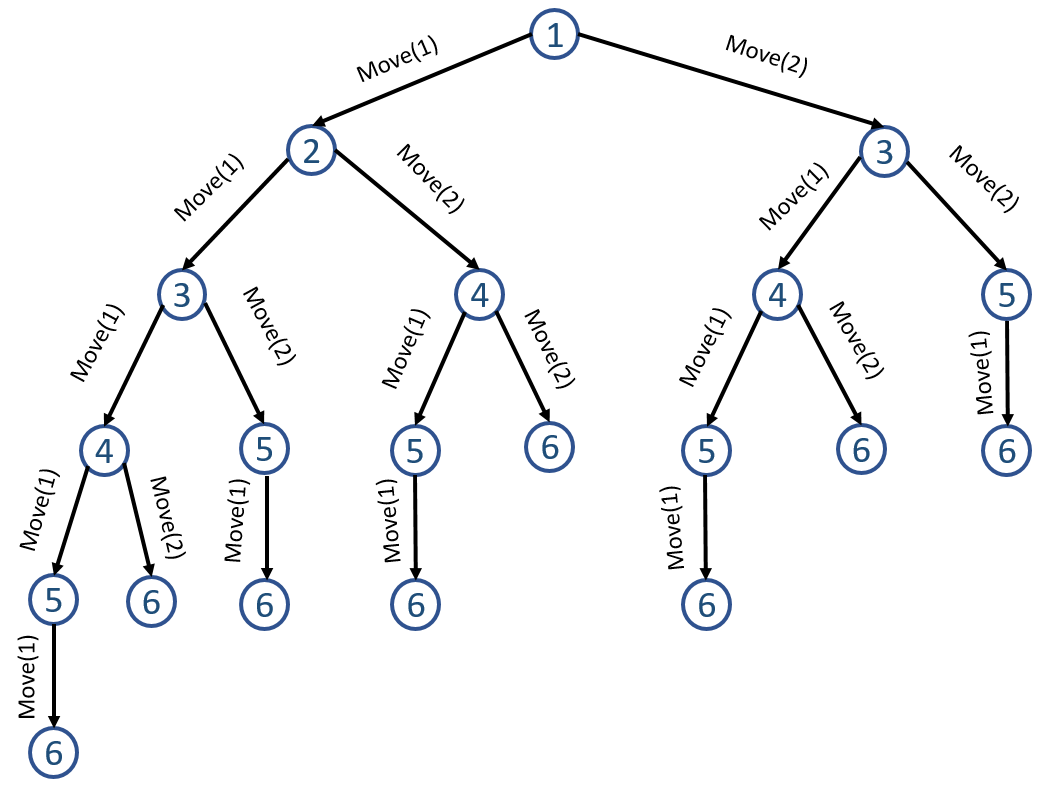
\includegraphics[width=0.7\columnwidth]{fig/problem_formulation_2.png}
    \caption{The State Space Graph. This may appears as a tree, but we can redraw it as a graph. }
    \label{fig:problem_formulation}
\end{figure}
 
\begin{enumerate}
    \item \textbf{Initial State:} state that where our algorithm starts. In our example, we can scan the whole list starting from leftmost position 0, we denote it as $S(0)$. Note that a state does not equal to a point on the input instance, it can be a range --such as from position 0 to 5, or from 0 to 2, or any state you define. 
    \item \textbf{Actions or MOVES:} describe possible actions relating to a state. Now, given position 1 with 2 as value, we can move only one step forward and get to position 2 or we can move 2, 3, 4, 5 steps and so. Thus, we should find all possible actions or moves that we can take to progress to next state. We can denote it as ACTIONS(1)={MOVE(1), MOVE(2), MOVE(3), MOVE(4), MOVE(5)}. 
    
    \item \textbf{State transfer Model}: decides the state results from doing an action $a$ at state $s$. We denote it as $T(a, s)$. For example, if we are at position 1 and move one step, MOVE(1), then we can reach to state 2, which can be denote as $2=T(MOVE(1), 1)$. %We also use the term \textit{successor} to refer to any state reachable from a given state by a single action. 
    
   \item \textbf{State Space:} is the set of all states reachable from the initial state by any sequence of actions, in our case, it can be {0, 1, 2, 3, 4, 5}. We can infer state space of the problem from the initial state, actions, and transfer model. The state space forms a directed network or \textit{graph} in which the nodes are states and the links between nodes are actions. Graph, with all its flexibity, is a universal and natural way to represent relations. For example, if we limit the maximum moves we can make at each state to two, the state space will be formed as follows in Fig.~\ref{fig:problem_formulation}. In practice, draw the graph as a tree structure is another option; in the tree, we observe repeat states due to the expansion of nodes in graph with multiple ingoing links.  A \textit{path} in the state space is a sequence of states connected by a sequence of actions. 
    
    
   \item  \textbf{Goal Test:} the determines whether a given state is a goal state. %Sometimes there is an explicit set of possible goal states, and the test simply checks whether the given state is one of them. 
   Such as in this example, the goal state is $4$. The goal is not limited to such enumerated sets of states, it can also be specified by an abstract property. For example, in the constraint state problems(CSP) such as the n-queen, the goal is to reach to a state that not a single pair of queens will attack each other. 
\end{enumerate}

In this example, the space graph is an analysis tool; we use it to represent the transition relationship between different states not the exact data structure that we use to operate and define algorithms on. 

\paragraph{Apply Data Structures}
\begin{figure}[!ht]
    \centering
    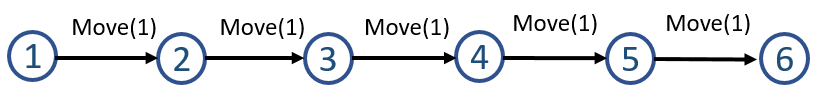
\includegraphics[width=0.9\columnwidth]{fig/problem_formulation_1.png}
    \caption{State Transfer process on a linear structure }
    \label{fig:problem_formulation_1}
\end{figure}

With the state space graph, our problem is abstracted to finding a node with value 4 and graph algorithms--more specifically, graph search--can be applied to solve the problem. It does not take an expert to tell us, "This graph just complicated the situation, because our intuition can lead us to a much simpler and straightforward solution: scan the items from the leftmost to the rightmost one by one". True! As is depicted in Fig.~\ref{fig:problem_formulation_1}, the problem can be modeled using a linear structure, possiblly a list or linked list, and we only need to consider one action out of all options, MOVE(1), then our searching covers the whole state space, which makes the algorithm we designed \textit{complete}~\footnote{Check complexity analysis}. On the other side, in the state space graph, if we insist on moving two steps each time, we would not be able to cover the whole state space, and might end up not finding our target, which indicates this algorithm is \textit{incomplete}.
\begin{figure}[!ht]
    \centering
    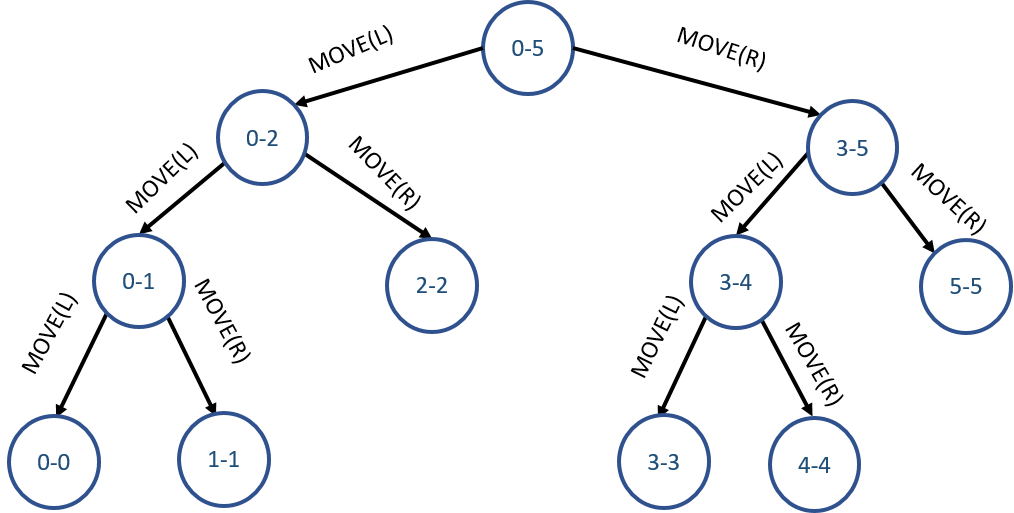
\includegraphics[width=0.7\columnwidth]{fig/problem_formulation_3.png}
    % 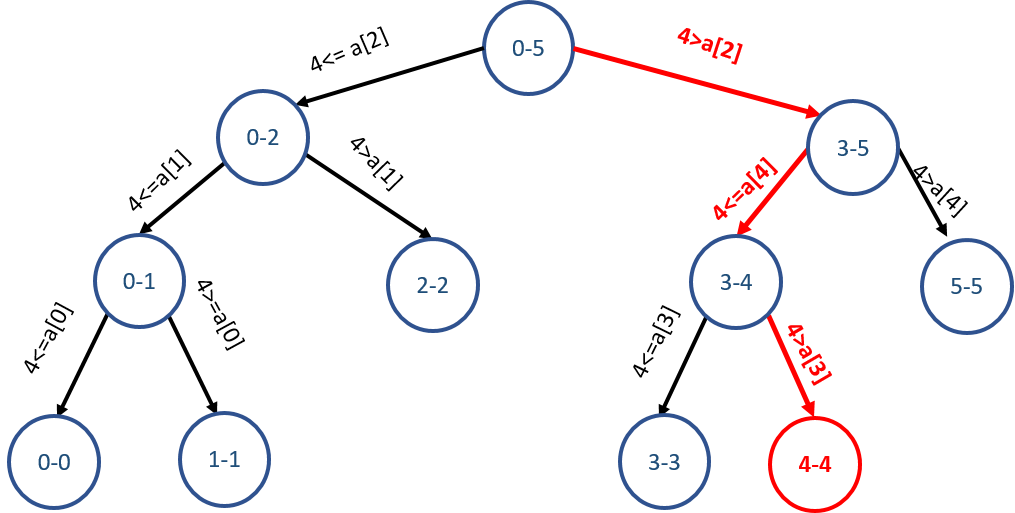
\includegraphics[width=0.7\columnwidth]{fig/problem_formulation_4.png}
    \caption{State Transfer Process on the tree}
    \label{fig:problem_formulation_2}
\end{figure}



Instead of using linear data structure, we can restructure the states as a tree if we refine the state as a range of items. The initial state  is the possible subarray the target can be found, denote as $S(0, 5)$. Start from initial state, each time, we divide the space into two halves: $S(s, m)$ and $S(m, e)$, where $s, e$ is the start and end index respectively, and $m=(s+e)//2$, meaning the integer part of $s+e$ divided by 2. We do this to all nodes repeatedly, and we will have another state transfer graph shown in Fig.~\ref{fig:problem_formulation_2}.From this graph we can see, the last node will be where we can not divide further, that is when $s=e$. From state $0-5$ to $3-5$ needs an action--move to the right. Similarly, from $0-5$ to $0-3$ needs the action of moving to the left.  We use {MOVE(L), MOVE(R)} to denote the whole set of possible actions to take.

In this example, we showed how to same simple problem can be modeled using two different data structures--linked list and tree. 




%we introduce the definition and the type of data structures; and demonstrate how it can be used to model our problems.   of data structures as a way to demonstrate our organization of part.~\ref{part_data_structure} and a premise knowledge for the next section where we examine and discuss the problem modeling with real examples.

% \subsubsection{Data Structures Definition}

% \subsubsection{Data Structures Categorizes} Put figures here for visualization and comparison. 
% \begin{enumerate}
%     \item Linear Data Structure: such as arrays, strings, heaps, priority queue.
%     \item Non-linear Data structure: such as tree, graph
%     \item Sturcutual: points, polygons. 
% \end{enumerate}

% Throughout this book, we will see that all problems are associated with fundamental data structures such as array, strings, trees, graphs, points, polygons. With different data structure, specific algorithms will be applied to solve these two problems. Data Structure is a way of collecting and organizing data in such a way that we can perform operations on these data in an effective way. Data Structures is about rendering data elements in terms of some relationship, for better organization and storage. \textit{In practice, data structures are utilized to model a problem so that it can be solved with a corresponding algorithm. }

% \textit{Data strutures and algorithms are inseparable in computer programming. }

% In order to do comparison between all possible devised algorithms for our problem, we need to learn how to  evaluate their performance with time complexity and space complexity. There are some techniques we will introduce before we dive into the four problem solving paradigm and Cracking LeetCode Problems (Part~\ref{part_cracking_leetcode_problem}), we will learn how to do complexity analysis of algorithms in Section~\ref{sec_complexity_analysis}. 




% The above example is to show us, how learning and practice using the data structures and four problem solving paradigms can help us making smarter decision about problem modeling and problem solving. 

\section{Problem Solving}
\label{sec_problem_solving}
In this section, we will first demonstrate how algorithm can be applied on these two data structures with its corresponding state transfer process. Following this, we introduce the four fundamental algorithm design and analysis methodologies--the ``soul/brain''.
 We end this section by briefing on categorizing algorithms. 
 
 \subsection{Apply Design Principle} 
\begin{figure}[!ht]
    \centering
    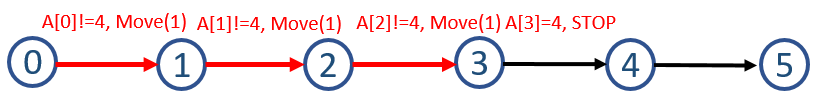
\includegraphics[width=0.9\columnwidth]{fig/problem_formulation_1_1.png}
    \caption{Linear Search on explicit linear data structure }
    \label{fig:problem_formulation_3}
\end{figure}
Given the state transfer graph in Fig.~\ref{fig:problem_formulation_1}, we simply iterate each state and compare each item with our target to see if it equals; if true, we find our target and return, if not, we continue to the end. This simple search method is depicted in Fig.~\ref{fig:problem_formulation_3}.
\begin{figure}[!ht]
    \centering
    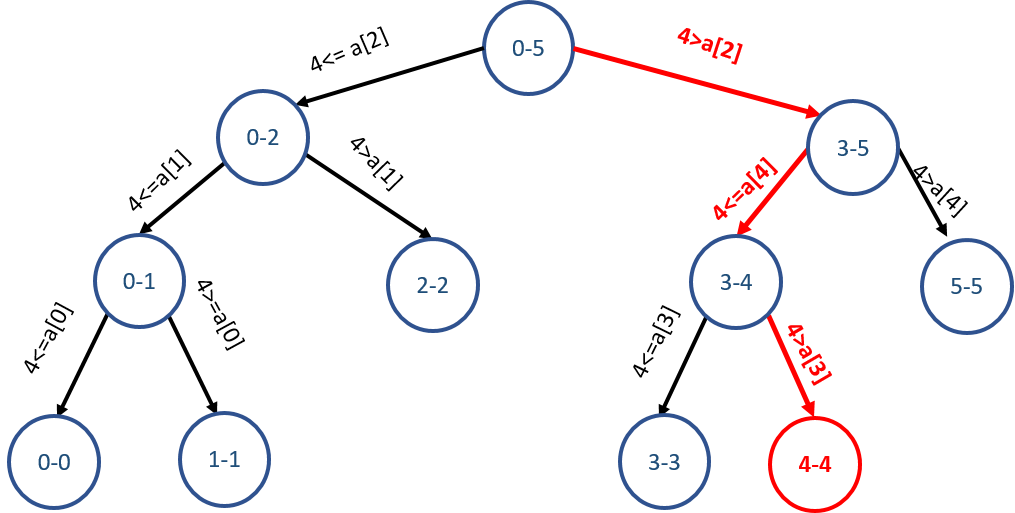
\includegraphics[width=0.7\columnwidth]{fig/problem_formulation_4.png}
    \caption{Binary Search on an implicit Tree Structure}
    \label{fig:problem_formulation_4}
\end{figure}
What if we know that the data is already organized in ascending order? With the tree data structure, when given a specific target, we only need to choose one action from the actions set; either move to left or right to search with a condition: if target is larger or smaller than the item in the middle of the state. When 4 is target, we have the search process depicted in  Fig.~\ref{fig:problem_formulation_4}. 

All these state space, data structure, algorithm, and analysis might appear overwhelming to you for now. But as you learn, some of these steps are not necessary, but knowing these elements are good for you to analyze and learn new algorithms, think of it more gathering terminologies into your language base. 

\subsection{Algorithm Design and Analysis Principles}
\subsubsection{Algorithm Design}
\label{sec_algorithm_design}
More of the time, the most naive and inefficient solution -- \textit{brute-force solution} would strike us right away, which is simply searching a feasible solution  to the problem in its solution space using the massive computation power of the hardware. Although the naive solution is not preferred by your boss nor it will be incorporated into the real product, it offers the baseline for your complexity comparison and to showcase how good your well-designed algorithm is.

In the dummy example, we actually used two different searching algorithms--linear search and binary search. The process of looking for a sequence of actions that reaches the goal is called search. Therefore, \textit{searching} is the fundamental strategy and and the very first step to problem-solving. How could it not be? Algorithms are about to find answers to problems, if and assuming we can define out potential state/solution space, then a naive/exhuastive searching would do the magic and solve the problem. However, back to reality, we are limited by computation resource and speed, we comprise by:
\begin{enumerate}
    \item being smarter that we can be decrease the cost, increase the speed, and yet still gives out the exact solution we are looking for. This comes down to \textit{optimization}, which we have \textit{divide and conquer}(Chapter~\ref{}), \textit{dynamic programming}(Chapter~\ref{}), and \textit{greedy algorithms}(Chapter~\ref{}). What are the commonality between them? They all in some way need us to get \textit{recurrence relation}((Chapter~\ref{}), which is essentially \textit{mathematical induction}(Chapter~\ref{}), which I generalized from another book, \textit{Introduction to Algorithms: A Creative Approach}, by Udi Manber. Explain it in another way, these principles are using recurrence relation to find the relation of a problem with its smaller instance. Why is it smarter? First, smaller problems are just easier to solve than larger problems. Second, the cost of assembling the answer to smaller problems to answers to the larger problems is possibly smaller.
    \item by approximating the answer. Instead of trying to get the exact answer, we find one that is good enough. Here goes to all heuristic search, machine learning, artificial intelligence. Guess, currently my limited knowledge is not enough for me to give more context that this.
\end{enumerate}
Equally, we can say all algorithms can be described and categorized as searching algorithms. Yet, there are three algorithm design paradigms-- \textit{Divide and Conquer}, \textit{Dynamic Programming}, and \textit{greedy Algorithms}, can be applied in the searching process for faster speed or using less space. 
Don't worry, this is just the introduction chapter, all these concepts and algorithm design principles will be explained later.

% \subsubsection{Algorithm Design Methodologies}
% In this section we will briefly offer a glimpse into their concepts and discerns. 
% \begin{figure}[h]
%     \centering
%     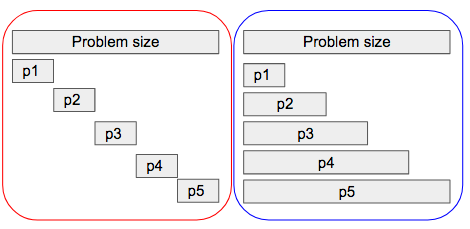
\includegraphics[width=0.6\columnwidth]{fig/divide_dynamic.png}
%     \caption{The dividing of problems of Divide and Conquer VS Dynamic programming. (Note: the left side in the red box is the Divide and Conquer, and the blue box is the dynamic programming.) }
%     \label{fig:divide_conquer_vs_dynamic_programming}
% \end{figure}

% \paragraph{Divide and Conquer} is the most fundamental programming philosopy.  It first recursively break a problem into smaller non-overlapping subproblems till a small base subproblem which can be solved easilty, and then combining the results of the subproblems into the solution to its superme problem in some way. The process is demonstrated in Fig~\ref{fig:divide_conquer_vs_dynamic_programming}, and it usually be implemented with recursive function. It usually decrease the time complexity of logarithm level. For instance, it optimize a $O(n^2)$ time complexity to $O(n\log n)$.


% \paragraph{Dynamic programming} follows the same philosophy of Divide and Conquer and commonly used to tackle optimization problems. It also first break a problem into subproblems. But instead of the non-overlapping subproblems, their subproblems overlaps in a way as demonstrated in Fig~\ref{fig:divide_conquer_vs_dynamic_programming}, which means a larger size subproblem grows from smaller previous subproblems. The solution to current subproblem can depends on any number of previous smaller subproblems.  With dynamic programming, intermediate results are cached and can be used in subsequent operations. 
% %Second, we use the knowledge we learned from normal algorithm books with algorithm methodology like divide and conquer, dynamic programming, greedy algorithms and so on. This normally be more efficient, if we are pick the right method. There methods will be introduced in details in Part~\ref{part_algorithms}. 

% \paragraph{Greedy algorithms} often involve optimization and combinatorial problems; the classic example is applying it to the traveling salesperson problem, where a greedy approach always chooses the closest destination first. This shortest path strategy involves finding the best solution to a local problem in the hope that this will lead to a global solution.

% \textcolor{red}{\paragraph{Complete Search} Complete search, also known as brute force or recursive backtracking, is a method for approaching a problem by naively searching through the whole solution spaces to obtain the required solution. Optimization is through pruning the searching space by ending invalid searching early. Complete search is used when there is clearly no clever algorithms available ( algorithms that use one of previous three paradigms), for instance with permutation and combination stated in Section~\ref{sec_combination}, or when such clever algorithms exist, but overkill when the input size happen to be small for complete search. }

% On the LeetCode, a lot of times, complete search should be the first considered soltion that come to mind. With bug-free complete search solution, we should never receive Wrong Answer response, but we might get Time Limited Error (TLE) instead due to its high time complexity. 

\subsubsection{Algorithm Analysis of Performance}
How to measure problem-solving performance? Up till now, we have some basic ways to solve the problem, we need to consider the criteria that might be used to measure them. We can evaluate an algorithm's performance in four ways:
\begin{enumerate}
    \item \textbf{Completeness:} Is the algorithm guaranteed to find a solution when there is one?
    \item \textbf{Optimality:} Does the stategy find the optimal solution, as defined?
    \item \textbf{Time Complexity:} How long does it take to find a solution?
    \item \textbf{Space Complexity:} How much memory is needed to perform the search?
\end{enumerate}

Time and space complexity are always considered with respect to some measure of the problem difficulty. In theoretical computer science, the typical measure is the size of the state space graph, |V | + |E|, where V is the set of vertices (nodes) of the graph and E is the set of edges (links). This is appropriate when the graph is an explicit data structure that is input to the search program. However, in reality, it is better to describe the search tree that applied to search for our solutions. For this reason, complexity can be expressed in terms of three quantities: $b$, the \textbf{branching factor} or a maximum number of successors of any node; $d$, the \textbf{depth} if the shallowest goal node ; and $m$, the maximum length of any path in the state space. Time is often measured in terms of the number of nodes in the search tree, and the space are in terms of the maximum number of nodes stored in memory. 

For the most part we describe time and space complexity for search on a tree; for a graph, the answer depends on how ``redundant" paths  or ``loops" in the state space are.


\subsection{Algorithm Categorization}
There are countless algorithms invented, however, these traditional data-independent algorithms (not the current data-oriented deep learning models which are trained with data), it is important for us to be able to categorize the algorithms and understand the similarities and characteristics of each type and also be able to compare each type: 
\begin{itemize}
    \item By implementation: the most useful in our book is recursive and iterative. Understand the difference of these two, and the special usage of recursion (Chapter~\ref{chapter_iteration_recursion}) is fundamental to the further study of algorithm design.  We can also have serial and parallel/distributed, deterministic and non-deterministic algorithms. In our book, all the algorithms we learn are  serial and deterministic algorithms. 
    \item By design: algorithms can be interpreted to one or several of the four fundamental problem solving paradigms, Divide and Conquer (Part~\ref{part_divide_conquer}), Dynamic Programming and Greedy (Part~\ref{part_dp_greedy}).  In Section~\ref{four_paradigm}, we will briefly introduce and compare these four problem solving paradigms to gain a global picture of the spirit of algorithms. 
    \item By complexity: mostly algorithms can be categorized by its time complexity. Given an input size of $n$, we normally have categories of $O(1)$, $O(\log n)$, $O(n\log n)$, $O(n^2)$, $O(n^3)$, $O(2^n)$, and $O(n!)$. More details and the comparison is given in Section~\ref{complexity_subsec_cheat_sheet}.
\end{itemize}
% \subsubsection{Searching Algorithms}
% After the problem formulation, we will have a sense of state spaces, and to reach to the goal state, we need to search a path to reach to this state or a sequence of actions. Searching algorithms will be the most fundamental footstone of all algorithms. Essentially our state spaces are graphs. Under certain limitations, we can simplify it to linear data structure or tree structures.  

% \paragraph{How searching works?} We start from the initial state and form a \textit{search tree} with the initial state as root; the branches are actions and the nodes corresponds to states in the state space of the problem. We search by \textit{expanding} current state; that is, applying each legal action to the current state, thereby reaching to a new set of states. The nodes available for expansion at any given point is called the \textbf{frontiers} (also called open list). There are fundamentally three types searching techniques:
% \begin{enumerate}
%     \item Breath-first Search: for example, if we are at 1, then our next sets of states are {2, 3}. Then we expand the states of 2, then states of 3, and save them to a data structures to expand later, they will be {3, 4, 4, 5}. So first, the frontier is {1}, then it becomes {2, 3}, then at node 2, we expand 3, 4, will end up with {3, 3, 4}. This is called breath-first search which expand the frontier in a First-in, first out or FIFO fashion (FIFO queue). Breath-first search is usually implemented iteratively. 
    
%     \item Depth-first Search: similarily at state 1, we get our frontiers to be {2, 3}. But if we deal with the nodes in the frontier in a last-in, first out or LIFO fashion (LIFO queue and also known as stack). At node 1, our generated frontier will be [2, 3], then we go to state 3, and expand more states here, the resulting frontier will be [2, 4, 5]. Then move to state 5, with resulting frontier [2, 4, 6]. Depth-first search can either be implemented iteratively or recursively. 
    
%     \item Priority based Search: if we pop the elements of the queue with the highest priority according to some ordering function, this is called proprity based search, this can be implemented with a priority queue. 
% \end{enumerate}



The intractable problems are still get solved by computer. We can limit our input instance size. However, it is not very practical, when the size of the input size is large and we are still hoping to get solutions, maybe not the best, but are good enough in a a reasonable(polynomial) time.   \textit{Approximate algorithms} comes into our hand,  such as \textit{heuristic algorithm}. In this book, we focus more on the non-approximate algorithmic methods to solve problems in \textit{discrete} solution spaces, and only brief on the part of approximate algorithms. 




%%%%%%%%%%%%%%%%%%%%%%%%%%%%%%%%%%%%%%%%%%%%%%%%%%%%%
\section{Programming Languages}
\label{sec_programming_languages}
 



hird, for certain type of problems, there are algorithms specically designed and tuned to optimize that type of question. This wil be introduced in Part~\ref{part_specific_algorithms}. Which might give us almost the best efficiency we can find.

% The fourth level, is the ''clever'' way. For some problems, if you are creative enough, and you comprehensively analyze the problem and think about each case, we might come up with a very brilliant solution that beats all the previous solutions in both efficiency and code elegancy. This will not be systematically introduced in this book, because it varies problem to problem. But we will put some ``clever'' solutions to some problems either in examples or exercises used in this book. 
% \subsection{Complete Search}

% \subsection{Divide and Conquer}
% \subsection{Dynamic Programming}
% \subsection{Greedy Algorithm}

\section{Tips for Algorithm Design}
\paragraph{Principle} 
\begin{enumerate}
    \item Understand the problem, analyze with searching and combinatorics to get the complexity of the naive solution.
    \item If it is a exponential problem, check if the dynamic programming applies. If not, we have to stick to a search algorithm. If it applies, we can decrease the complexity to polynomial. 
    \item If it is polynomial already or polynomial after the dynamic programming applied, check if the greedy approach or the divide and conquer can be applied to further decrease the polynomial complexity. For example, if it is $O(n^2)$, divide and conquer might decrease it to $O(n\log n)$, and the greedy approach might end up with $O(n)$. 
    \item If none of these design principle applies: we stick to the searching and try to optimize with better searching techniques--such as backtracking, bidirectional search, $A^{*}$, sliding window and so on. 
\end{enumerate}
This process can be generalized with ``BUD''--bottleneck, unncessary work, and D. 



\section{Exercise}
\subsection{Knowledge Check}
\paragraph{Longest Increasing Subsequence} 


\begin{bclogo}[couleur = blue!30, arrondi=0.1,logo=\bccrayon,ombre=true]{Practice first before you check up the solution. (put the solution at next page)}
\end{bclogo}
\begin{figure}[!ht]
    \centering
    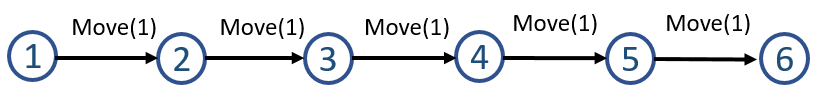
\includegraphics[width=0.9\columnwidth]{fig/problem_formulation_1.png}
    
     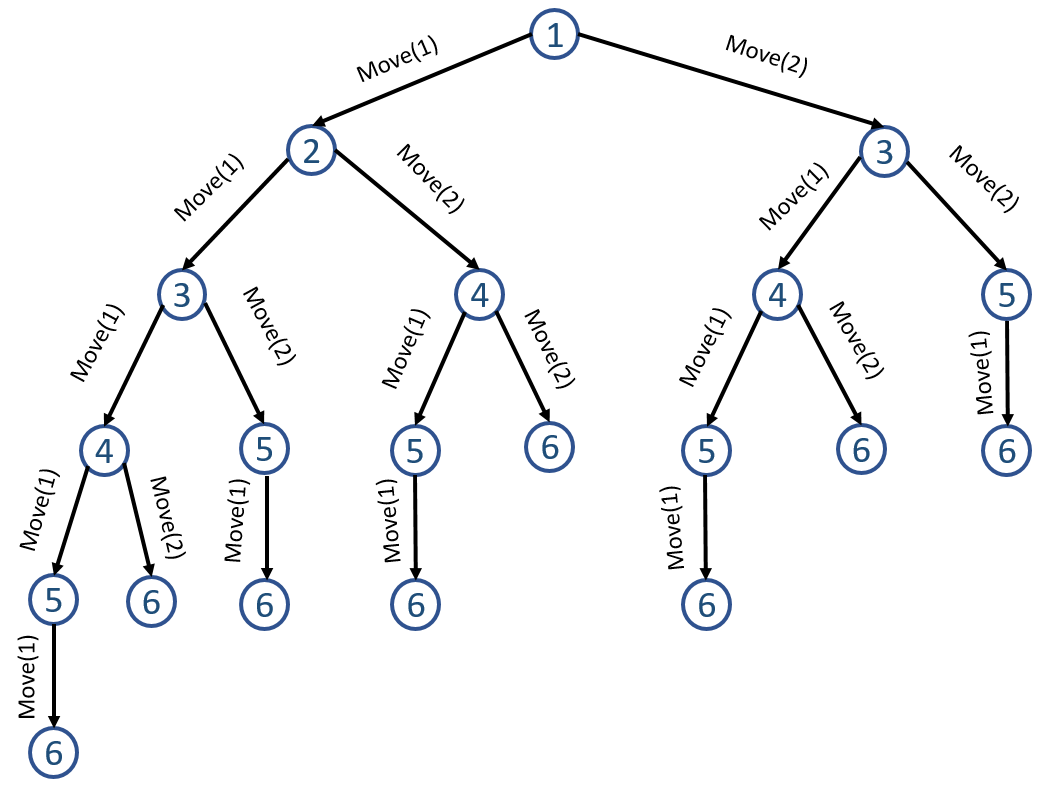
\includegraphics[width=0.7\columnwidth]{fig/problem_formulation_2.png}
    \caption{The State Spaces Graph }
    \label{fig:problem_formulation}
\end{figure}
 Given a list of items $A=[1, 2, 3, 4, 5, 6]$, find the position of item with value $4$. 
\begin{enumerate}
    \item \textbf{Initial State:} state that where our algorithm starts. In our example, we can scan the whole list starting from leftmost position 1. $S(0)$
    \item \textbf{Actions or MOVES:} A description of possible actions available at a state. If we are at position 1, we can have different possible actions, we can move only one step forward and get to position 2. Or we can move 2, 3, 4, 5 steps. We can denote it as ACTIONS(1)={MOVE(1), MOVE(2), MOVE(3), MOVE(4), MOVE(5)}. 
    
    \item \textbf{State transfer or transition model}: It returns the state results from doing an action $a$ at state $s$. We denote it as T(a, s). For example, if we are at position 1 and take action that move one step, MOVE(1), then we can reach to state 2, denote as $2=T(MOVE(1), 1)$. We also use the term \textbf{successor} to refer to any state reachable from a given state by a single action. 
    
  \item \textbf{State Space:} Together, the initial state,  actions, and transition model implicitly define the state space of the problem--the set of all states reachable from the initial state by any sequence of actions. The state space forms a directed network or \textbf{graph} in which the nodes are states and the links between nodes are actions. For example, if we limit the maximum moves we can make at each state to be one and two, the state space will be formed as follows in Fig.~\ref{fig:problem_formulation}. A \textbf{path} in the state space is a sequence of states connected by a sequence of actions. 
    
    
  \item  \textbf{Goal Test:} the goal test determines whether a given state is a goal state. Sometimes there is an explicit set of possible goal states, and the test simply checks whether the given state is one of them. Such as in this example, the goal state is $4$. Sometimes the goal is specified by an abstract property rather than explicitly enumerated sets of states. For example, in the constraint state problems(CSP) such as the n-queen, the goal is to reach to a state that not a single pair of queens will attack each other. 
\end{enumerate}


In practice, analyzing and solving a problem is not answering a yes or no question. There are always mutiple angels to model a problem, the way to model and formalize a problem decides the corresponding algorithm that can be used to solve this problem. And it might also decide the efficiency and difficulty to solve the problem. For example, using the Longest Increasing Subsequence:
\begin{figure}[h]
    \centering
    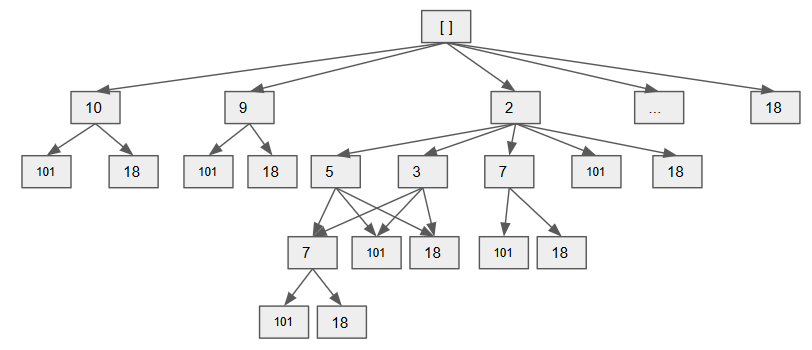
\includegraphics[width=\columnwidth]{fig/LIS_tree.png}
    \caption{State Transfer Tree Structure for LIS, each path represents a possible solution. Each arrow represents an move: find an element in the following elements that's larger than the current node.}
    \label{fig:tree_lis}
\end{figure}
\textbf{Ways to model the problem.} There are different ways to model this LIS problem, including:
\begin{enumerate}
    \item Model the problem as a directed graph, where each node is the elements of the array, and an edge $\mu$ to $v$ means node $v>\mu$. The problem now becomes finding the longest path from any node to any node in this directed graph.  
    \item Model the problem as a tree. The tree starts from empty root node, at each level i, the tree has n-i possible children: nums[i+1], nums[i+2], ..., nums[n-1]. There will only be an edge if the child's value is larger than its parent. Or we can model the tree as a multi-choice tree: for combination problem, each element can either be chosen or not chosen. We would end up with two branch, and the nodes would become a path of the LIS, therefore, the longest LIS exist at the leaf nodes which has the longest length.
    \item Model it with divide and conquer and optimal substructure. 
\end{enumerate}

\end{document}